\documentclass[letterpaper,11pt]{article}

%packages
\usepackage{amsfonts}
\usepackage{graphicx}
\usepackage[left=2cm,top=2cm,right=2cm,bottom=1.5cm,head=.5cm,foot=.5cm]{geometry}
\usepackage{url}
\usepackage{multirow}
\usepackage{longtable}
\usepackage{subfig}
\usepackage{float}
\usepackage{setspace}
\usepackage{lineno}
\usepackage{natbib}
\usepackage{amsmath}
\usepackage{authblk}
\usepackage{xr}
\usepackage{relsize}
\usepackage{tikz}
\usepackage{hyperref}

%new commands and so on
\providecommand{\keywords}[1]
{
  \small	
  \textbf{\textit{Keywords---}} #1
}

\DeclareMathOperator{\E}{\mathbb{E}}% expected value
\DeclareMathOperator{\var}{var}
\DeclareMathOperator{\cov}{cov}
\DeclareMathOperator{\cor}{cor}
\DeclareMathOperator{\mean}{mean}
\DeclareMathOperator{\se}{se}
\DeclareMathOperator{\sd}{sd}
\DeclareMathOperator{\prob}{P}

%attempt 1 at nat and sharp
%\newcommand{\nat}{\mathlarger{\natural}}
%\newcommand{\shp}{\mathlarger{\sharp}}

%attempt 2 at nat and sharp
%\newcommand{\nat}{\raisebox{1pt}{\mathsmaller{\mathsmaller{/\hspace{-2pt}/}}}}
%\newcommand{\shp}{\#}

%attempt 3 at nat and sharp
\newcommand{\nat}{%
\text{\hspace{-1.5pt}
\begin{tikzpicture}[scale=1.8]%
\draw (.333ex,0) -- (.333ex,1ex);%
\draw (.666ex,0) -- (.666ex,1ex);
\end{tikzpicture}%
}}
\newcommand{\shp}{%
\text{\hspace{-1.5pt}
\begin{tikzpicture}[scale=1.8]%
\draw (0,.333ex) -- (1ex,.333ex);%
\draw (0,.666ex) -- (1ex,.666ex);%
\draw (.333ex,0) -- (.333ex,1ex);%
\draw (.666ex,0) -- (.666ex,1ex);
\end{tikzpicture}%
}}
\newcommand{\test}{%
\text{
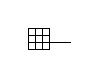
\begin{tikzpicture}[scale=1.8]%
\draw (0,0) -- (1ex,0ex);
\draw (0,0) -- (0ex,1ex);
\draw (0,1ex) -- (1ex,1ex);
\draw (1ex,0) -- (1ex,1ex);
\draw (0,.333ex) -- (2ex,.333ex);%
\draw (0,.666ex) -- (1ex,.666ex);%
\draw (.333ex,0) -- (.333ex,1ex);%
\draw (.666ex,0) -- (.666ex,1ex);
\end{tikzpicture}%
}}

\newcommand{\olr}{\overline{r}}
\newcommand{\olrs}{\overline{r}^{\shp}}
\newcommand{\olrn}{\overline{r}^{\nat}}
\newcommand{\bs}{\backslash}
\newcommand{\olep}{\overline{\epsilon}}

%header material for paper
\title{Responses to referees for ``Asymmetric relationships and their effects on coexistence''}
\date{July 2023}

\begin{document}

\noindent \emph{Dear Editors,} \\

\noindent \emph{Thank you for the useful and very positive reviews of our manuscript, and for
the opportunity to resubmit a revised version. We have addressed all referee comments below and in
the manuscript, and hope the paper can now be rapidly accepted. } \\

\noindent \emph{We have replied to referee comments below in italic, with each response preceded
by ``***'', to make our responses easier to find.} \\

\noindent \emph{We submit the following pdf files: ...} \\
%DAN: Fill in ...

\noindent \emph{We additionally submit the following latex files, necessary for compiling the
main text latex: ...} \\
%DAN: Fill in ...

\noindent \emph{The document showing the changes we made does not include links such as citations and
references to figures, but it does accurately represent the changes made to the text. 
If all latex files are deposited into the same folder, it should then be possible to 
compile the main text latex from that folder.} \\

\noindent \emph{We again thank the referees and editors for their feedback and positive reviews!} \\

\noindent \emph{Yours,}

\noindent \emph{Dan Reuman and Jasmin Albert} \\

\noindent \textbf{Comments of referee 1:} \\

\noindent C1) This is a very interesting paper that adds to our understanding of modern coexistence theory through the decomposition of the ways in which competitive pressure and environment can be correlated.\\

\noindent ***\emph{Thank you for the positive feedback!} \\
%DONE

\noindent C2) Specifically, the focus is on asymmetric tail association (ATA), by which two random variables with given, fixed marginal distributions and correlation can nevertheless differ in the way that their right and left tails are correlated. This is one among many ways that one could characterize or decompose the full bivariate distribution between competition and environment, but the authors argue and demonstrate that ATAs of this kind are (a) prevalent in natural systems and (b) can have a meaningful and sometimes qualitative effect on the outcome of coexistence between two species.  The combination of results for theoretical distirbutions but also for experimental data is very powerful and convincing. \\

\noindent ***\emph{Thank you for the positive feedback!} \\
%DONE

\noindent C3) I have one overarching question, which I think may be important for ensuring that those points (a) and (b) are robust and then some minor comments that may improve the readability of the manuscript for the EL audience. \\

\noindent ***\emph{We address your questions and comments below.} \\
%DONE

\noindent C4) My biggest question is related to the removal of ATAs from a given true bivariate distribution.  This is described in SI Section S2 and shown visually for an example in SI Figure S1. 

My first comment related to this is that some form of this text (whcih is relatively short---around half a page in the SI) and, importantly, the Figure should be in the main text.  I think this is such a key part of the definitions that are being used for the rest of the paper that readers will want to get an intuition for what the "partial sharp" distributions look like and how they are arrived at. \\

\noindent ***\emph{We have done what the referee requests, here, and we agree with this request. Thanks for
making the request. This request is somewhat in tension with other requests, from other referees, 
to minimize the quantitative 
content of the main text, and to keep the overall length under the journal limit while adding a bunch of
verbal explanations requested by the other referees. We point out this tension here, and refer back to it in
other responses, below. We also point out that we have not only moved the figure back to the main text,
we have also added a panel to the figure in response to the related comment C13, below.} \\
%DONE
%DAN: In other replies, you can refer to this reply to justify when you
%decide to add explanations to the SI instead of to the main text, and when you have to respond to requests
%to minimize the quant. 

\noindent C5) Perhaps equally important to clarifying this process for the readership is whether this process is unique. I could not quite get a sense of whether there could be alternative versions of this removal of ATA from a bivariate distribution, that still satisfy the authors' constraints on marginal distributions and overall correlation between the two variables. Are there alternatives, or is the authors' procedure unique in achieving the desired outcome?  If the former, then I would want to understand if the outcomes downstream tend to be robust to the specific method used. If the latter, it would be helpful to have an explanation as to why this is a unique decomposition. \\

\noindent ***\emph{This is a good question, thanks for asking it. The extent to which the process is 
unique is now covered in a new SI section, refered to from the main text at the end of section 2.3, 
right at the end of the text the referee asked us to move to the main text. There is a choice involved,
but it is pretty canonical -- certainly more canonical than the kinds of choices which are often made
in MCT, e.g., $E$ and $C$ can sometimes be defined in more than one way. Basically the choice involves 
using a bivariate normal distribution instead of another, more esoteric 
distribution with standard normal marginals and symmetric tail association. The bivariate normal is by far the 
most natural example of such a distribution. See the new SI section for further explanations. }

\emph{We are reticent, at this time, to launch into a lot of robustness explorations with regard to this choice, 
as the referee may be suggesting, for several reasons. First, other referees and the editor have urged us to
simplify, and such explorations would complexify instead. Second, as mentioned above, the choice we made is very
natural and quite standard, so exploring other possible choices seems therefore of 
secondary importance. Finally, our overall goal in writing this paper
was to show that ATAs may be important for coexistence and, as such, deserve additional exploration in this
context by the wider research community. As long as any choices we made are reasonable (they are), our point is
made, regardless of whether making some more esoteric choices might have altered outcomes. As we already argue in the
Discussion, since we have now showed that ATAs \textbf{can} be important, future work should explore \textbf{when} 
they are important, and part of 
that exploration could be whether some more esoteric choice for $(e_i c_{i \bs i})$ might alter our results. }\\
%DONE

\noindent C6) The notation by which the partial sharp variables are introduced was a little unintuitive to me.  For example, when the authors compare the expectation values 
$E[r(E,C)]$ and $E[r(E^{||},C^{||})]$, what is really changing is the distribution over which the expectation values are evaluated.  Maybe this is standard notation, but somehow it may be clearer to put the subscript on the E for expectation value, to indicate that the probability distribution used to generate the definition of the averaging is what differs between the two expressions, while the variables E and C themselves are in the end just dummy variables to be integrated over.  \\

\noindent ***\emph{This comment has led us to put some clarifying technical comments in a new SI section 2,
so thanks for making the comment.} 

\emph{We use notational conventions of random variables which are formally correct and standard, 
as we now explain in more detail in the SI. 
$E_i$, $C_{i \bs i}$, $E_i^{\nat}$, $C_{i \bs i}^\nat$ and the earlier 
notation $E_i^\shp$ and $C_{i \bs i}^\shp$ all denote \textbf{random variables}, using a 
notational approach which is standard in applications of probability. 
Whereas the \textbf{distributions} of the random variables $E_i$, $E_i^{\nat}$ and $E_i^\shp$ (for instance) are all the same,
these things are \textbf{not} the same \textbf{as random variables} because their relationships with other random variables 
differ. The relationships between random variables are considered instrinsic
to the notation. Thus it's not that somehow the expected value in $\E[r(E,C)]$ is a different definition of expected
value than the one in $\E[r(E^{||},C^{||})]$ -- there is only one expected value operator. 
Instead, $r(E,C)$, $r(E^{||},C^{||})$ and $r(E^\shp,C^\shp)$ differ from each other 
as random variables because of the distinct relationships between their
different $E$ and $C$ constituents. It would be formally 
incorrect, and confusing to readers familiar with probability, to try to define multiple expected value 
operators, as the referee seems to suggest, when what fundamentally differs, here, is the random variables 
themselves. Readers familiar with
probability already know what the one accepted definition of expected value is, would typically
not be comfortable with providing additional definitions, and are comfortable handling these concepts
with the notational conventions we have used. To remind the referee of some concepts from basic probability
which illustrate these conventions, recall that if $X$ and $Y$ are random variables, the expectation of the 
product, $\E(XY)$, depends not only on the univariate distributions of $X$ and $Y$, but also on the relationship
between $X$ and $Y$, namely their joint distribution. In particular, $\E(XY)=\E(X)\E(Y)$ if $X$ and 
$Y$ are independent, but not necessarily otherwise. These definitons and notation are completely 
standard in probability theory; notice that we use the same definition of $\E$ regardless of 
whether $X$ and $Y$ are independent or nonindependent, it's just that the product random variable
$XY$ differs accordingly so you get different results of $\E(XY)$ in those distinct cases.}

\emph{Our notation also parallels that of Ellner et al (2016, 2019). To make it
easier for readers to understand and to reduce the potential for future confusion, it makes sense to continue
using existing notation whenever that notation is formally correct and otherwise effective (it is, as explained above).}

\emph{Nevertheless, the referee's comment has made us understand that some readers unfamiliar with random variable 
notation may benefit from putting some
of these explanations in the SI, so we have done so.} \\
%DONE

\noindent C7) It was not clear to me what the reasoning was for including the correlation and ATAs in abundance for the two planktonic species in Figure 1(d) and (e).  These ATAs in abundances don't in an obvious (to me) way translate into ATAs of the underlying environment and competition variables for each species. Is this really a demonstration that ATAs occur for C and E?  If not, then it seems to be like saying ATAs exist somewhere in nature, and therefore might be present in our focal situation, which is not such a very strong reason to show (d) and (e).  Maybe I am missing something. \\

\noindent ***\emph{Yes, the referee is right about this, we are not illustrating ATAs in $E$ and $C$ at this stage of the 
paper - the reader would anyway not be equiped to handle that at this stage, since we have not even formally defined 
$E$ and $C$ at the point this figure is first cited (in the very first paragraph). 
We were asked to include this kind of empirical illustration 
by poeple who read the manuscript before we submitted it, so it seems important to some readers to have this. 
The value is not only in showing that ATAs occur in nature, but is priarily  
in helping people understand more fully what they look like when they occur by giving real examples. 
We appreciate what the referee is saying,
here, that perhaps one non-$EC$ example of ATAs from nature is not going
to give much motivation for looking for ATAs in $E$ and $C$. However, we have published droves of other examples of
ATAs in nature, and we now cite these (changing what used to be ``Fig. 1d,e show contrasting examples of ATAs in nature
using plankton population density time series'' to ``Fig. 1d,e show contrasting examples of ATAs in nature
using plankton population density time series; and many other examples have also been previously explored (Ghosh et al 2020)''). 
And anyway we cannot produce a prior example of ATAs between $E$ and $C$ because there are no prior examples - this paper 
is, to our
knowledge, the first time anyone has looked at ATAs between $E$ and $C$. Fortunately, we think the other motivational
content of the Introduction is strong, and should stand on its own to motivate readers to spend their mental 
energy reading this paper. In partcular, we show in the Introduction, for one simple simulation, that ATAs between E and
C make a visually striking difference between simulation outcomes that appears clearly to influence coexistence.} \\
%DONE

\noindent C8) The authors mention that $r_{i \bs i}$ indicates growth rate of species when $i$ is rare and $j$ is at steady state.  I think $r_{j \bs i}$ must also assume that $j$ is at steady state, but this isn't mentioned. Perhaps that could be added for completeness. \\

\noindent ***\emph{This was done already, the referee appears to have missed it. It was line 136 in the original submission,
now line XXX in the resubmitted version.} \\
%Don't forget to add the new line numbers at the end.

\noindent C9) E.g. line 100 needs removal of the word "are" or the addition of the word "and" somewhere to make sense. I'd consider going through the paper carefully for any typos or small corrections of this kind. \\

\noindent ***\emph{We changed the wording as requested, and went through the entire manuscript again looking for typos
and grammatical errors.} \\
%Jasmin to look at line 100 and revise as needed. 

\noindent \textbf{Comments of referee 2:} \\

\noindent C10) In their paper the authors decompose the “storage effect” into two separate effects, what they call the “asymmetric tail association” and the covariance term per se. The authors explain well why they do this and why they think this may be important. Additionally, they show the best possible efforts to convince the readers why such a decomposition may be important and what we may learn from it. Overall, the paper is interesting and quite understandable. I think the authors have done a very good job. \\

\noindent ***\emph{Thank you for the very positive feedback!} \\
%DONE

\noindent C11) Unfortunately, I’m personally not convinced that storage effect (and therefore probably ATA) are relevant for coexistence in nature and therefore I’m sceptical about this new approach. I want to be clear that this is, in part, my personal opinion and I know experts in the field which have a very different view. What the authors have shown (and it appears to be correct) is that in a model where niche differentiation via different resources and predators is impossible, then ATA can be an important driver of coexistence, and I agree. However, in every application where both storage effect, relative non-linearity and niche differentiation have been measured, there we see that storage effect and relative non-linearity where very small compared to simple resource differentiation. But, one might argue, that we have barely any such empirical applications, and I would agree, which is why I label this my personal opinion. (The few papers that I know of are \href{https://nam10.safelinks.protection.outlook.com/?url=https%3A%2F%2Fdoi.org%2F10.1002%2Fecy.2726&data=05%7C01%7Cd294r143%40ku.edu%7C13ab816eaf2a49c27ea808db784a67cf%7C3c176536afe643f5b96636feabbe3c1a%7C0%7C0%7C638236033192197676%7CUnknown%7CTWFpbGZsb3d8eyJWIjoiMC4wLjAwMDAiLCJQIjoiV2luMzIiLCJBTiI6Ik1haWwiLCJXVCI6Mn0%3D%7C3000%7C%7C%7C&sdata=HbUTjzCNQrvGSARY5u3Eqme88DbKiNyiAVNOUGzjcbE%3D&reserved=0}{Zepeda et al. 2019, Ecology}, \href{https://nam10.safelinks.protection.outlook.com/?url=https%3A%2F%2Fdoi.org%2F10.1890%2F14-1741.1&data=05%7C01%7Cd294r143%40ku.edu%7C13ab816eaf2a49c27ea808db784a67cf%7C3c176536afe643f5b96636feabbe3c1a%7C0%7C0%7C638236033192197676%7CUnknown%7CTWFpbGZsb3d8eyJWIjoiMC4wLjAwMDAiLCJQIjoiV2luMzIiLCJBTiI6Ik1haWwiLCJXVCI6Mn0%3D%7C3000%7C%7C%7C&sdata=KKIBuLjBN2vNGWfEpduAGGrMAt7ov9a4F53CmlZQlO0%3D&reserved=0}{Chu and Adler 2015}, and Ellner et al. 2019, see also the new paper by \href{https://nam10.safelinks.protection.outlook.com/?url=https%3A%2F%2Fesajournals.onlinelibrary.wiley.com%2Fdoi%2Fepdf%2F10.1002%2Fecm.1585&data=05%7C01%7Cd294r143%40ku.edu%7C13ab816eaf2a49c27ea808db784a67cf%7C3c176536afe643f5b96636feabbe3c1a%7C0%7C0%7C638236033192197676%7CUnknown%7CTWFpbGZsb3d8eyJWIjoiMC4wLjAwMDAiLCJQIjoiV2luMzIiLCJBTiI6Ik1haWwiLCJXVCI6Mn0%3D%7C3000%7C%7C%7C&sdata=YaqsZ6axu6rYV12kh9IiRIbES7ZUMWIN7HXgB08iPzc%3D&reserved=0}{Stump and Vasseur}, which I have not yet read fully) In my understanding, ATA is a decomposition of storage effect into even more components, therefore I would expect, on average the ATA effect to be slightly smaller than storage effect (but, as you have shown can also be larger than storage effect). I would therefore assume that ATA is generally weak compared to niche differentiation (but again, admittedly based on few datapoints). Obviously, the authors may disagree with my personal view, in this case I’d like to see a discussion of this. \\

\noindent ***\emph{We thank the referee for this viewpoint. We also thank the referee for acknowledging that this
is their opinion, and that data are insufficient for a clear conclusion to be reached at this point. We find that 
such an acknowledgment is both rare from a referee and very useful for causing us, as authors, to most usefully revise our 
paper. We have added new discussion material covering these topics and find that the new material improves the paper.
We tried to represent both viewpoints in the new material, and we cited the papers the referee mentions.}

\emph{We point out that we worked not only
with the lottery model, but also with an empirical diatom system. That system definitely supported the importance of 
ATAs for coexistance, which would tend to give at least one data point in favor of the importance of these phenomena, though we 
acknowledge that our lab systems is also a system ``where niche differentiation via ... predators is impossible.''
It may also be a system ``where niche differentiation via different resources ... is impossible,'' though resource 
differentiation can happen when you don't expect it. It seems to us 
the first step in assessing the importance of a newly recognized phenomenon has to be examining it in simple systems
such as we have used, prior to examing it in field systems, in all their complexity, where niche differentiation
by resources and predators can more readily occur. But once our paper is published we hope and expect that we and
others will more broadly assess the potential importance of ATAs.}

\emph{We also point
out (and the referee already seems to accept this) that it is possible, \emph{a priori}, for ATAs to be 
important for coexistence in a system even while storage effects are not.
Storage effects are ATA effects plus what we called, in the manuscript, the effects of $EC$ correlation \emph{per se} 
($\Delta_i^{[E \nat C]}$ in our notation). Either of these two summands can be negative or positive.
So if the two effects are opposite in sign and similar in magnitude, storage effects will be unimportant for 
coexistence, but ATA effects will be important.}

\emph{So the referee appears to agree with us that storage effects and ATA effects may or may not turn
out to be broadly important in ecology. Our research goals were to introduce the idea of ATA effects on
coexistence and to show that ATAs \textbf{may} be broadly important for coexistence, by showing examples where they
\textbf{are} important. The few examples we showed are all that are readily available at this time.
We won't know for sure if ATAs (or storage effects) \textbf{are} important until more data can be brought to bear. 
Future work can assess, broadly, how important ATAs are by looking across a larger number of systems, once
available. These are two different goals. It seems crucial to us not to allow insufficiently tested 
opinions about the second set of goals to obstruct the publication of results pertinent to the first set of 
goals, so we thank the referee for not doing that. We modified a few key points in the text to clarify 
our viewpoint that we do not think our work definitively indicates that ATAs will certainly be a crucial
mechanism of coexistence; instead we just think our work opens that possibility, for future exploration.
For instance, we replaced the last sentence of the first paragraph of the Discussion, which used to be
``Though future work should seek to understand precisely when ATAs are or are not important
for coexistence, our work demonstrates the overall importance of this new mechanism'' with the revision
``Future work should seek to understand precisely when ATAs are or are not important
for coexistence. Our work demonstrates the potential for ATAs to be an important mechanism of coexistence, generally.''
And we changed the last sentence of the abstract, which used to read ``ATA influences are an important new 
mechanism of coexistence'' so that it now reads ``ATA influences may be an important new mechanism of coexistence.''
We think these changes make the paper stronger, so thanks for spurring us to make them. The last
sentence of the Introduction already read ``Overall, our study presents a new mechanism of species coexistence
and a means of understanding its theoretical and empirical importance,'' which accurately reflects our belief
that what we've accomplished is an indication that ATAs \textbf{may} be important for coexistence, 
and a means of assessing
that in future work, rather than a definitive conclusion that they are important for coexistence.}

\emph{The new Discussion material is in an SI section which is cited from the main text Discussion section. 
We would have liked to put some of the new material into the main text. But length limits, together with
clear requests from other referees to add a variety of content to the main text, made doing so impossible.} \\
%DONE

\noindent C12) I like the conceptual idea of removing the long tail. \\

\noindent ***\emph{Thank you for the positive feedback.} \\
%DONE

\noindent C13) However, I have somewhat difficulties to precisely understand/be sure I correctly understood what this does. I suggest you move a simpler version of Fig S1 into the main text and show the actual distribution, the uncorrelated distribution of $E$ and $C$, but same marginal distribution, and the distribution with the same covariance, but the ATA removed. Additionally, it might be beneficial to indicate which distribution is then used to compute which part of the decomposition. For example, in Figure S1 d you show $E_i^{||}$, but from my understanding this distribution would be used to compute $E_i^{(EC)}$, correct? \\

\noindent ***\emph{In comment C4 above, another referee asked us also to put S1 back into the main text, so
we have done as the referee asks here. The new Fig. 2 has the three elements the referee asks for, here, as 
its panels (a), (e) and (d). We retained the other panels as well, since those were requested by the 
other referee. Regarding the second part of the referee's comments, 
there is nothing in our paper for which the notation $E_i^{(EC)}$ is used, but we think what the referee must
be requesting here is what we remind the reader that $(E_i^\shp,C_{i \bs i}^\shp)$ is used to compute storage effects,
$\Delta_i^{(EC)}$, and that $(E_i^\nat,C_{i \bs i}^\nat)$ is used to compute ATA effects, $\Delta_i^{[EC]}$. We have 
now added such a reminder to the figure caption.} \\
%DONE

\noindent C14) You focus solely on storage effect with the argument that it’s the only where ATA can actually occur. But on a broader level you essentially decompose the EC distribution into it’s different momentums. One only carrying about the mean (i.e. first order correct), one with only carrying about the mean and covariance (i.e. getting the first two orders correct), and one with all other orders correct. Given this interpretation of your work, I might apply the same logic to the relative-nonlinearity, where I decompose the relative non-linearity into the variance term and the term with long tails. (one might also even decompose the actual distribution into more distributions, getting successively more and more momentums of the distribution correct, but I would argue that this is probably less useful). \\

\noindent ***\emph{We are not sure we understand precisely what the referee is saying here because their language
appears more suggestive than formally correct. Perhaps they mean
``moment'' rather than ``momentum''? Perhaps they mean ``caring'' instead of ``carrying''? I think the phrase 
``term with long tails'' does not precisely relate to what we're doing since marginal distributions
of the bivariate distribution $(E,C)$ are unchanged in all our approaches, and hence tails are unchanged. 
It's just relationships
between $E$ and $C$ that are modified in the different scenarios we consider. The referee's ideas, here,
if made precise, may be about potentially using a series of approximations to the bivariate distribution $(E,C)$
that have the same marginals as $(E,C)$ itself, but that get successively more co-moments right, compared to the
co-moments of $(E,C)$ itself (and the 
remaining co-moments would be zero, we presume, if
such distributions can be defined). Such an approach, applied to relative nonlinearity, would not give
anything interesting because relative nonlinearity only depends on the marginal distributions, which, 
under this framework, are always equal to the original marginals of $(E,C)$. On the other hand,
perhaps the referee means to take a series of approximations of $(E,C)$ so that the $n$th 
approximate distribution gets both moments and co-moments of order $\leq n$ right, with remaining
moments and co-moments zero (if such distributions can be defined). That may be interesting, but would
certainly be a different paper from ours, since our paper is about \emph{relationships} between $E$ and $C$
(while leaving the univariate distributions of $E$ and $C$ themselves fixed), whereas this idea of the 
referee would make approximations
both to the relationship between $E$ and $C$ and to the marginals, simultaneously. Nevertheless, 
we are pleased the referee 
is interested in our approach to the extent that they are generating potential ideas for future research.} \\
%DONE

\noindent C15) L34: I found this sentence confusing due to the two “betweens” and it’s not immediately clear to what they “bound” \\

\noindent ***\emph{We modified the sentence.} \\
%DONE

\noindent C16) L41: The “we” is slightly confusing because the author teams share only one author \\

\noindent ***\emph{We changed the wording here.} \\
%DONE

\noindent C17) L48: I do not know these on the top of my head, and likely many other readers will neither, so maybe quickly refresh our memory \\

\noindent ***\emph{There is no space to intro these things, so we limited this text to just mentioning 
extinction risks and stability of ecosystem functioning. Whereas some ecologists may not have heard of 
Taylor's law, we feel confident that extinction risks and stability of ecosystem functioning will ring
a bell for most ecologists. It was not actually necessary to link to Taylor's law, we just though it 
would provide an additional tie-in to another part of the literature. But that won't work if the referee is right 
that most ecologists will become confused, so we were happy to drop that connection here.} \\
%DONE

\noindent C18) L49: This is not immediately clear to me why (obviously, you’ve shown this in the other paper). Is it possible to briefly state why? \\

\noindent ***\emph{It is not necessary for the reader to understand the mechanism we explored in that other
paper in order to understand this current paper, we were just trying to tie the current work in to 
another area of research in ecology, for the sake of contextualizing it a bit and motivating studies of ATAs generally. 
So an explanation, here, is not 
strictly necessary to the current paper. Nevertheless, we tried to satisfy the referee's request of adding a bit of explanation
without disrupting the flow too much. Thanks for your interest, by the way, we encourage you to have a look at the
other paper if you haven't already.} \\
%DONE

\noindent C19) L61: What if not? Or many readers have only rough understanding of it, maybe quickly refresh or refer to later \\

\noindent ***\emph{It is not necessary for the reader to understand what these are at this point, and,
in fact, the reader does not need to understand what relative nonlinearity is at all for the main text
and main ideas of the paper. We apologize for giving the false impression, here, that more background knowledge was needed
than is actually the case. We eliminated the reference to relative nonlinearity and indicated to the 
reader that storage effects would be conceptually reviewed below (a couple paragraphs down) and then 
defined in Theory, which they are.} \\
%DONE

\noindent C20) Sidenote: After writing these few comments it appears to me that you seem to have a very knowledgeable reader in mind, which may not be the case for a general journal as Ecology letters. \\

\noindent ***\emph{Well, we appreciate the referee's effort to spur us to produce the clearest 
paper possible, and we have used the comments to clarify. But, of the comments 
C16-C19 above, only C19 relates at all to whether this paper is written for a general ecological audience,
and we have revised the text C19 mentions so as to robustly address that comment (see response above). 
The manuscript text mentioned in C17-C18 was just linking this paper to other prior work on ATAs. 
It's not necessary for the reader to understand that work to understand this paper, the point is just to make 
the link to that other literature, so that readers can explore it if they so choose, 
and to show that ATAs have been found to be important in ecology, generally, to motivate the study.
Furthermore, we don't think our paper is any more specialized or mathematical than the papers Ellner et al (2016, 2019) which
we cite, and which inspired our paper, and which were published in Ecology Letters. Nor is it more 
specialized than many other papers we have read in Ecology Letters. Quantitive approaches are absolutely 
central in ecology these days, and increasingly so. So comments which would tend to sideline such paper
"specialist journals", which fewer people read, seem outdated to us, especially when the papers in question 
are about mainstream topics such
as coexistence. Nevertheless, we have gone through the paper and redoubled our efforts to make the 
paper broadly accessible.} \\
%We have to go through the paper and redoubled our efforts to make the paper broadly accessible.

\noindent C21) L64: Narwani 2013 is actually not a good reference because it did not include any temporal variation, a better one would be Letten et al. 2019 in PNAS. \\

\noindent ***\emph{We replaced the reference.} \\
%Jasmin can you please do this?   %%REPLACED  

\noindent C22) L74: The optimum might actually be the same, but they need different responses. \\

\noindent ***\emph{Thanks for pointing this out, we have corrected our language.} \\
%DONE

\noindent C23) Eq. 1: I would not use any equations in the introduction, and in general this part of the introduction did not feel like an introduction at all and might require a different sub-section \\

\noindent ***\emph{We disagree, and would prefer not to make this change, for several reasons. 
First, the lottery model is a very simple model, at the same level of complexity
as models introduced in essentially all introductory 
undergraduate ecology courses (e.g., the Lotka-Volterra competition model), so there is no argument that 
the readership of Ecology Letters cannot easily understand the material presented here.
Second, this material serves a clear motivating purpose, most appropriately placed in the Introduction. 
The last author (DCR) has found, from decades of pitching 
quantitative papers to general ecological audiences, that clear motivation is essential - it is crucial to demonstrate 
clearly that an effect one plans to elaborate is present, and potentially important, prior to asking the reader to engage 
the kind of mental energy necessary to read the guts of the paper. So this 
paragraph is for showing that the effect of ATAs on coexistence can be real, at least for a simple 
example. That goal is convincingly 
accomplished by the paragraph, more so than could be accomplished by a purely qualitative, words-only Introduction. 
Given that the math is simple, and also more precise and definitive than 
qualitative verbal arguments, we think this material is actually
more beneficial to the readership and more effective for the intended motivational purpose than would be more words
(and we see based on C25 below that the referee appears to agree with us here in some respects, at least). 
Third, quantitative approaches are central in ecology these days, and increasingly so. The automatic tendency
to want to exclude mathematics of any kind from the Introduction, especially when the math is simple,
accessible, and serves a clear motivational purpose, seems like a dated bias to us. 
Finally, we firmly believe that ecology as a discipline gets stronger as it continues the clear
trend of the last few decades of incorporating more quantitative approaches. We believe we
benefit the field by challenging assumptions and biases such as categorically not putting equations 
in the Introduction.} \\
%Jasmin to read the above and let Dan know if it's convincing or not, and how it can be improved.
%It's done except for any improvements or revisions that Jasmin may suggest.
%Jasmin: I really like this response and don't think its too harsh or needs to be toned down. 

\noindent C24) L93: I suggest ``Note that $N = N_1(t) + N_2(T)$ is constant through time''. \\

\noindent ***\emph{OK, we made this change, even though the same equation already appears just a few lines
above this spot. Perhaps the referee is right that the reminder will benefit some readers.} \\
%DONE

\noindent C25) L95-99: I think this is a great teaser to get the readers to later dive in into your mathematics \\

\noindent ***\emph{Thank you! This is exactly our purpose, here, and we are pleased it has been effective.
Relating back to our response to C23, we think this purpose cannot really be convincingly accomplished
without first stating the lottery model, since the result uses that model. Math is more precise and can be
more convincing than language, the trade off being that some readers won't understand some math. However, the 
math we have in the Intro is so simple we think all readers of Ecology Letters will understand it, so there are
benefits and basically no costs of including it there. } \\
%DONE

\noindent C26) L126: Do you do this in the appendix? \\

\noindent ***\emph{No. We can see how it would be done, but we have not formalized the mathematics. 
To avoid making claims that we have not fully supported
with rigorous mathematics, we rephrased to say the iid assumption is 
``probably not necessary''. Thanks for spurring us to do this.} \\
%DONE

\noindent C27) Eq 2.: I thought we also have to remove the effect of C varying alone and E varying alone? Is this included in the $\#$ term automatically? \\

\noindent ***\emph{No, the equation is correct as is. Please see equation 10 and related equations of 
Ellner et al, 2019, Ecology Letters. Yes, the effects of $C$ and $E$ varying are included in 
the $\#$ term because that terms involves both of them varying (though independently).}

\emph{Also, see our SI section ``Mechanisms other than storage effects". 
%can delete if not needed
Since,
\begin{align}
\olep_i^{EC} &= \E[r_i(E_i,C_{i \bs i})]-\olep_i^E-\olep_i^C-\epsilon_i^0 \\
&= \olr_{i \bs i} - \olep_i^E - \olep_i^C - \epsilon_i^0,
\end{align}
and 
\begin{align}
\olep_i^{(E\shp C)} &= \E[r_i(E_i^\shp,C^\shp_{i \bs i})]-\olep_i^E-\olep_i^C-\epsilon_i^0 \\
&= \olrs_{i \bs i} - \olep_i^E - \olep_i^C - \epsilon_i^0,
\end{align}
we have
\begin{align}
\olep_i^{(EC)} &= \olep_i^{EC}-\olep_i^{(E\shp C)} \\
&= (\olr_{i \bs i} - \olep_i^E - \olep_i^C - \epsilon_i^0) - (\olrs_{i \bs i} - \olep_i^E - \olep_i^C - \epsilon_i^0) \\
&= \olr_{i \bs i} - \olep_i^E - \olep_i^C - \epsilon_i^0 - \olrs_{i \bs i} + \olep_i^E + \olep_i^C + \epsilon_i^0 \\
&= \olr_{i \bs i} - \olrs_{i \bs i}. 
\end{align}
So,
\begin{align}
\Delta_i^{(EC)} &= \olep_i^{(EC)} - q_{ij}\olep_j^{(EC)} \\
&= (\olr_{i \bs i} - \olrs_{i \bs i}) - q_{ij}(\olr_{j \bs i} - \olrs_{j \bs i}) \\
&= \olr_{i \bs i} - \olrs_{i \bs i} - q_{ij}\olr_{j \bs i} + q_{ij}\olrs_{j \bs i} \\
&= \olr_{i \bs i} - q_{ij}\olr_{j \bs i} - \olrs_{i \bs i} + q_{ij}\olrs_{j \bs i} \\
&= (\olr_{i \bs i} - q_{ij}\olr_{j \bs i}) - (\olrs_{i \bs i} - q_{ij}\olrs_{j \bs i}),.
\end{align} 
which is the equation the referee is asking about.} \\
%DONE

\noindent C28) Eq. 6: Maybe highlight that you use different brackets ([EC] versus (EC)), or probably even better, make 5 and 6 one equation using curly under brackets. \\

\noindent ***\emph{Yes, it is a good idea to make it completely clear to the reader that these are 
used distinctly. We now do so, though we do it above this point in the text - it is better, in our view,
to do this the first time we use the hard brackets. So thanks for pointing this out.
We do not know what the referee means by ``using curly under brackets'' so have not done anything
in response to that part of this comment.} \\
%DONE

\noindent C29) L230 $\mu_1-\mu_2$ is negative, why not take $\mu_2-\mu_1$? \\

\noindent ***\emph{Well, we can do this if the editor insists, but to us, avoiding the use of
negative numbers is insufficient reason to have to undertake the substantial and time-consuming 
work, and potential for error, 
of re-doing several figures, and revising many formulas (in the main text and SI) which currently use the other convention.
After all, negative numbers are basic, and represent no impediment to the average ecologist understanding the 
paper.} \\
%DONE

\noindent C30) L316: So why do you show values of $\sigma >6$? And also maybe highlight this in the figure Figure 1d and e: I’m semi convinced by these distributions showing ATA. In 1d it simply appears that the variance scales with the density. 1e is quite unconvincing to me. That’s generally fine, but figure 1 seems to be a conceptual figure, so I wonder whether you don’t have a better example? \\

\noindent ***\emph{Regarding the first referee question listed above, well, what we are 
trying to do here is accurately portray our results about
when ATAs were important and when they were not. To us, the most forthright way of doing that is to
show \textbf{all} the results, including the values of $\sigma$ which are probably unrealistic, and mention
(as we do) that some values are unrealistic. The point of this paragraph is to outline the circumstances
we have explored, using our lottery-model approaches, for which ATAs were important or not, and including all
our results seems important when such is our goal. Furthermore, there's no real cost to showing
all the $\sigma$'s we explored, it does not take up more manuscript space to do so.
Some readers may also take the lesson, for future work, from these explorations that one of the things that probably 
matters for continuing to explore when ATAs are important and when not is probably the strength
of the noise impacting the system. Finally, whether a value of $\sigma$ is ``unrealistic'' is 
a bit of judgement call rather than a formal cutoff, to we hesitate to censor results 
based on such a thing.}

\emph{Regarding the second part of the referee comment, pertaining to Figure 1d and e, it is perplexing to us that 
this is mentioned here,
as the paragraph at L316 is not directly related to Fig. 1d-e. That figure
shows motivational empirical examples, distinct from the lottery model work discussed around L316. Nevertheless, we took
seriously the referee's comment that they were apparently not convinced there are ATAs in Fig. 1d-e.
In fact, one can significance test these results and they are solidly significant - we added
those results, along with the methods used to get them, to a new SI section which is now cited from the
figure caption. We also added some text to the figure caption which we hope will focus the 
readers attention on the aspects of these panels which clearly show asymmetries of tail association. } \\
%DONE

\noindent C31) Figure 2: I recommend to add a line at $y = 0$. Also the different subgraphs have different $y$-scales which I’m not sure is beneficial, but unsure myself. \\

\noindent ***\emph{There is already a line at $y=0$. You can see it, for instance, on panel (e). 
It gets unavoidably overplotted on panels for which one of the plotted quantities is close to 0. The reason
for different $y$-axis extents is so that you can see the variation within each panel with maximum 
clarity. The main point, here, is to compare the relative contributions of different components
to coexistence, so it's important to show within-plot variation (between lines and across 
values of the $x$-axis) clearly. We tried plotting with the same scales everywhere and it obscured some of the 
patterns. We thank the referee for expressing their own uncertainty, which was
useful to be aware of.} \\
%DONE

\noindent C32) Figure 2 and 3: It appears that ATA is almost never the relevant factor, however I wonder whether this is because ATA is relatively weak, or whether the same analysis of say $\delta_i$ would lead to a similar pattern, it might be worth creating these graphs in the appendix to strengthen your case. \\

\noindent ***\emph{For Fig. 2, the referee is right that ATAs are only rarely important, as explained in the text 
(see first paragraph of section 4.1). However, for Fig 3, the referee is incorrect. In that figure, the ATA term
is usually one of the largest-magnitude contributions to coexistence. Our results as to the importance of ATAs for coexistence 
contrast between our log-normal and beta funcundities lottery models, as explained in the last paragraph
of section 4.1. That's one of the points we are making.} \\
%DONE

\noindent C33) Figure 2: ATA is always positive, so how can it lead to ATA exclusion? (or ATA rescue in case I misunderstood). \\

\noindent ***\emph{The referee appears to have misinterpreted the figure. The ATA terms is, in fact, usually
negative for this figure. The colors of lines corresponding to different terms are in the legend, and, in the caption,
it is reviewed which of these corresponds to the ATA term. Since these items are clearly labelled, and since 
the $y=0$ line is also already present, we are unsure how to reduce the chances for other readers to make
such errors. But we're happy to hear specific suggestions.} \\
%DONE

\noindent \textbf{Comments of referee 3:} \\
  
\noindent C34) This is a well performed paper pointing out that asymmetric tail associations (ATA) in a correlation between the environment and competition can be an important mechanisms of coexistence previously overlooked. ATAs can give additional mechanisms that either promote or hinder coexistence in a similar fashion and magnitude to other previously recognised mechanisms such as the storage effect. To illustrate these ideas the authors combine results from mathematical models, simulations, and empirical examples, and show that under a certain combination of parameters ATAs can be a significant mechanism of species coexistence. \\

\noindent ***\emph{Many thanks for the positive feedback!} \\
%DONE

\noindent C35) Overall, I agree with the authors that the role of ATAs in coexistence has not been properly considered and the manuscript give convincing results of the importance of ATAs. \\

\noindent ***\emph{Thank you for the positive feedback!} \\
%DONE

\noindent C36) However in order to reach a broad audience of ecologists, the manuscript needs to reach a balance between mathematical definitions and simple explanations. Otherwise, it can remain to technical and of little importance to ecologists interested in the role of environmental variability of community dynamics. I will give some examples where the message can be improved, but I would suggest the authors to do the same effort themselves in other parts of the manuscript. \\

\noindent ***\emph{We have gone to great lengths to address the referee's specific suggestions below, and we have also redoubled our
efforts to make the manuscript as accessible as possible, generally. We appreciate being spurred to do so, thanks. } \\
%We have to redouble our efforts, as it says. Maybe we also want to point out somewhere that this particular
%sub-field is already a very technical one, but is nevertheless considered a mainstream and very important
%area in ecology? %food webs? networks

%I wrote the following, but decided not to include it here. Might include it elsewhere:
%The research field
%surrounding the MCT and mechanisms of coexistence is very important within ecology, but is nevertheless technical - see, for instance, the
%papers of Chesson, which have had enormous positive impact on the field, as well as the recent papers of Ellner which helped inspire
%our paper. All those papers, and many other papers in the field, are unavoidably technical, but have frequently been published
%in mainstream journals (the Ellner papers are in Ecology Letters) because of their importance and the importance of the subject
%matter they investigate. Though we agree with all efforts to make research results as clear as possible to non-technical audiences,
%we beg the referee

\noindent C37) At the beginning of the introduction the authors cite previous work to show the prevalence and importance of ATAs for population dynamics, and the stability of ecological communities, and Fig.1 illustrate what ATAs mean in a clear example, yet it is not well explained or at least it was not clear to me how ATA can either promote or hinder coexistence in these initial sentences. \\

\noindent ***\emph{The referee appears to want us to present an intuitive explanation for how ATA effects work, and that 
is certainly a good idea. We have invested substantial efforts into doing so, and think we have succeeded. Though the referee's comment above may 
be interpreted to suggest that they wanted us
to add such an explanation to first paragraph of the paper, the reader is not equiped to understand the explanation at that 
point, so we added a new paragraph later in the Introduction (it is now the
second-to-last paragraph in the Introduction) that begins establishing such an intuition. We also added some text to the end of
the second paragraph that adds to the intuitive understanding of how ATAs can influence coexistence through a concrete 
example. We also added a new paragraph to the 
Discussion (the second paragraph of the Discussion). These new Discussion 
paragraphs are also supported by two new SI sections and two new SI figures which 
explain, in detail, how the intuition established in the two new main text paragraphs emerges from the modelling (SI sections S11 
and S12, SI Figs S4 and S5).
%DAN: make sure these are the final numbers of these SI sections
We believe that intuition such as the new material establishes should always be based in formal theoretical and 
empirical work, so the focus of the paper remains on our expansion of the MCT and our results showing
the *importance* of ATA effects. Though we definitely think our additions giving an intuition for ATA effects are a large
improvement in the manuscript, so we thank the referee for spurring us to make these additions.  } \\
%DONE except the checking as noted above.

\noindent C38) Then the explanation of the importance of ATAs is done in relationship with the explanation of the storage effect. In detail, the explanation of the storage effect is superb, ... \\

\noindent ***\emph{Thank you for the positive feedback! We have also added some text to the end of that paragraph giving a 
concrete case (water limitation) in which one may expect an influence of ATAs. We think the new text definitely
makes it more intuitive reasonable to explore ATA contributions to conexistence.} \\
%DONE

\noindent C39) ...but how ATAs enter in play is not well solved. It is just mentioned that ATAs can modify the EC covariation, which I believe is not enough, a reader might not understand later the explanation when the lottery model is presented. \\

\noindent ***\emph{See our response to C37. We have added substantial material to the Introduction and Discussion that adds an
intuitive explanation for ATAs, and we thank the referee for spurring us to do so. 
We find it unlikely that any focussed reader will have substantial difficulties understanding the lottery model
material in the Introduction, since the lottery model is certainly no more complicated than models such as the Lotka-Volterra 
competition and predator-prey models, which are covered in essentially every introductory undergraduate ecology class, and we can assume
that almost all readers of Ecology Letters have taken such a class. See also comment C25 above, which indicates that another
referee found this material to be compelling.} \\
%DONE

\noindent C40) ATAs can not only modify the importance of the storage effect but also of other mechanisms such as relative non-linearity, which is based on how competition fluctuates in ways that favor the competitor. Could the authors briefly indicate how this could occur? \\

\noindent ***\emph{This cannot occur. ATAs can only influence storage effects, not the other mechanisms, as stated at
the top of section 2.4 and explained mathematically in the SI section cited there. Basically, as explained in 2.4, 
this is because ATAs are about covariation between $E$ and $C$, whereas the mechanisms other than storage effects
do not pertain at all to covariation. For instance, relative nonlinearity is about the effects of variation 
in $E$ or $C$, not covariation between them.} \\
%DONE

\noindent C41) The lottery model is used to illustrate the importance of ATAs, and two types of fecundities are taken 
into account (log-normal and beta), can the author explain why both are important, and later on the results and discussion 
why ATAs play a major role with beta fecundities and not with log-normal.
The model used for the chemostat is in its formulation quite different compared to the lottery model. Although the technical
details are left for the supplementary material, can the authors explain more in the detail in the main text how the 
importance of ATAs can be used for this particular model.\\

\noindent ***\emph{This is certainly a valid question, and we have gone to substantial lengths to address it. 
Partly in response to this comment and partly in response to earlier comments of referee 3, 
we added substantial new material providing intuitive explanations of ATA effects in the Introduction,
Discussion, and SI (see above responses). That new material also has information comparing the models
and explaining why ATA effects are substantial for the beta-fecundities lottery model and not as strong
for the log-normal fecundities lottery model. These are very positive additions to the manuscript, so we 
thank the referee for spurring us to add them. We also believe this is only a start -- additional explanations and intuitive 
explorations of ATA effects could and should be the subject of future papers. We've added as much material 
as possible on these topics to the current manuscript, given length limits and
requests from the referees to both simplify and add a variety of other content.} \\
%DONE

\noindent C42) The chemostat model is parameterized with information from a previous study, but does this model reproduce observed dynamics of the diatom system? this needs to be shown otherwise the importance of ATAs will be considered for another dynamics that do not correspond to the observed ones. \\

\noindent ***\emph{response} \\
%I think the earlier papers already showed that, at least for the parameters used there? Check. And the other parameters
%are experimentally manipulable, so this should be OK, but is worth discussing the extent to which ATAs were important
%for the original parameters. The it would be worth noting that the strongest ATA contributions come for parameters
%which were not imposed in the original experiment, so it may be worth repeating the experiment but with these other
%parameters.

\noindent \textbf{Comments of the editor:} \\

\noindent C43) This study novelty is the focus on assymetric tail association between competition and environmental conditions as a mechanism of coexistence. \\

\noindent ***\emph{Thank you for pointing out the novelty.} \\

\noindent C44) The manuscript is very theoretical with a highly technical language hard to follow by a broad range of ecologists. My main suggestion is that the authors need to rewrite it in several parts to make it accessible and convincing. The authors have to make an effort to use a more biological/ecological language with reference to real world potential examples/cases/systems. Some mathematical material could be moved to Supplementary material. \\

%Need to address. However, this papers seems no more technical than the earlier Ellner paper. And, furthermore, 
%one of the referees (ref 1) actually asked us to put BACK technical content in the main text which we had 
%moved to the SI before submission to keep it less technical. Also, this research area is technical, though it
%is still central to ecology as a discipline. Recycle some of your arguments above about technical aspects. 
%That said, we do need to do a pass thu and figure out what technical content we can reduce, so we can make it
%as clear as it can be. Note also they say the math *could* be moved, suggesting less importance than 
%using ``a more biological/ecological language...''. So maybe let's try to do more of that, some of which
%I've alreday done thru answering the referee comments.
\noindent ***\emph{response} \\

\end{document}